\documentclass{article}
\usepackage[utf8]{inputenc}
\usepackage{hyperref}

\usepackage{url}
\usepackage{listings}
\usepackage[pass]{geometry}
% \usepackage{vmargin}
\usepackage{fancyhdr}
\usepackage{amsmath}
\usepackage{amsfonts,amssymb,amsthm,cite,float,graphicx}
\graphicspath{ {images/} }
% \usepackage[tight,footnotesize]{subfigure}
\usepackage[usenames]{color}
\usepackage{algorithm,algorithmic}
\usepackage{graphicx}
\usepackage{caption}
\usepackage{subcaption}
\usepackage{multicol}
\usepackage{float}
\usepackage{mathtools}


\title{Capturing Hysteresis in the Hodgkin-Huxley Model}
\author{Faris Sbahi and Stuart Ki}
\date{April 2017}

\begin{document}

\maketitle

\section{Introduction}

Alan Lloyd Hodgkin and Andrew Huxley, in 1963, won the Noble Prize in Physiology and Medicine for their work developing the Hodgkin-Huxley Equations, equations that modeled to incredible accuracy the propagation of action potentials through a squid axon. 

In our project, we seek to simplify and visualize the model while still capturing the important qualitative behaviors of the axon system. Specifically, we will first take experimental data to fix some parameters to constants, effectively lowering the dimension of the H-H model. Then, we will redact this assumption and attempt to exploit the fact that one of our variables is fast and the other is slow by using nullcline analysis. We will seek to show that this model performs well at indicating important qualities of the H-H model. Finally, we will attempt to follow FitzHugh\cite{FITZHUGH1961445} and capture those same qualitative behaviors in a yet simpler model by observing which specific characteristics actually produce the interesting properties. 

Of course, we must first develop the H-H model itself.

\section{Premises of the Hodgkin-Huxley Model}

The Hodgkin-Huxley model models the cell membrane as a simple circuit. 

\begin{figure}[h]
    \centering
    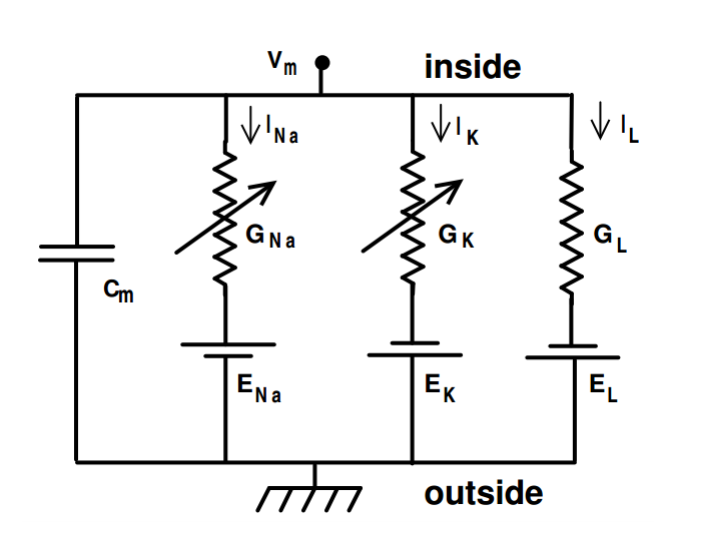
\includegraphics[scale=0.5]{hhmodel}
    \caption{Hodgkin-Huxley Circuit}
    \label{fig:my_label}
\end{figure}


Two voltage-dependent sodium and potassium channels allow the ions to flow through the membrane. The membrane has a capacitance indicated by $c_m$. Additionally, the sodium and potassium channels have a conductance parameter $G_{Na}$ and $G_K$, as well as a leakage conductance as shown. These conductance parameters can be modeled by various functions as will be shown later, and model the buildup in the passage of ions that create the action potential. The circuit is in parallel to mimic the axon. 

Using classic current conservation in a circuit, and adding the parameter of an external current $I_{ext}$, we can derive the current equation for the cell.

\begin{equation}
    c_m\frac{dV_m}{dt} + I_{ion} = I_{ext}
\end{equation}

In our particular model, we will assume that $G_L$ is constant and the capacitance $c_m$ as well. $V_m$ is the potential within the cell membrane, and $I_{ion}$ is the net ionic current within the cell.

The derivation of each ionic current through the different channels depends on the conductance parameter times the driving potential.

\begin{equation}
    I_{ion} = G_{ion}(V_{m}-E_{ion})
\end{equation}

Conductance is modeled in a certain way. The physical meaning of conductance is the probability that the channels that the ions pass through will be considered open, or when the gates that the ions can pass through are all permissive in that particular ion channel. This is dependent on the voltage of the cell membrane. 

Hodgkin and Huxley used three different types of gates to model the conductance channels. Using, $m$, $h$, and $n$ as different types of gates (iterations of $p$), $G_{Na}$ and $G_K$ are modeled as followed.

\begin{equation}
    G_{Na} = \bar{G}_{Na}m^3h
\end{equation}
\begin{equation}
    G_{K} = \bar{G}_{K}n^4
\end{equation}

Where $m$, $h$, and $n$ follow the following differential equation, which is derived on the open fraction of gates, $p$:

\begin{equation}
    \frac{dp}{dt} = a(V)(1-p) - b(V)p
\end{equation}

Hodgkin and Huxley discovered that as they kept the voltage constant, the conductance of the channels increased steadily to a maximum value. They used this experimental data to achieve equations for the time step of increase of $p$.

\begin{equation}
    p_{\infty}(V) = \frac{a_p(V)}{a_p(V) + b_p(V)}
\end{equation}
\begin{equation}
    \tau_p(V) = \frac{1}{a_p(V) + b_p(V)}
    \label{eq:time}
\end{equation}

Where $p_{\infty}(V)$ is the steady state value at an given voltage and ${\tau_p}(V)$ are time constants of response of the gates, in relation to $p$ growing to its steady state value. These constants can be experimentally fit to data and using Equation (5), $a_p(V)$ and $b_p(V)$ can be found. Thus, the final equations for the rate constants are as follows.

\begin{align*}
    a_m(V) &= \frac{0.1(25-V)}{\exp(\frac{25-V}{10})-1}
    &b_m(V) = 4e^{-V/18} \\
    a_n(V) &= \frac{0.01(10-V)}{\exp(\frac{10-V}{10})-1} 
    &b_n(V) = 0.125e^{\frac{-V}{80}}\\
    a_h(V) &= 0.07e^{\frac{-V}{20}} 
    &b_h(V) = \frac{1}{\frac{\exp(30-V)}{10}+1}
\end{align*}

We can also simplify equation 5 to the following.

\begin{equation}
    \frac{dp}{dt} = \frac{p_{\infty}(V)-p}{\tau_p(V)}
\end{equation}

The combined system of differential equations is shown in the next section. Furthermore, in Figure \ref{fig:inf} we show the values of $m_\infty$ and $n_\infty$ derived using the equations above. 

\begin{figure}
\centering
	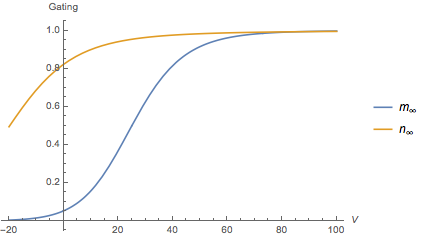
\includegraphics[height=5cm]{gating.png}
	\caption{$m_{\infty}$ (blue) and $n_{\infty}$ (orange)}
		\label{fig:inf}
\end{figure}

\section{Deriving a Reduced-State Model}

Evidently, the state variables for the model are $V$, $m$, $h$, and $n$. Hence, we can write

\begin{align*}
    C\frac{dV}{dt} &= I_{ext} -\bar{G}_{Na}m^3h(V-E_{Na}) -\bar{G}_{K}n^4(V-E_{K})  -\bar{G}_{L}m^3h(V-E_{L}) \\
    \frac{dm}{dt} &= \frac{m_{\infty}(V)-m}{\tau_m(V)} \\
    \frac{dh}{dt} &= \frac{h_{\infty}(V)-h}{\tau_h(V)} \\
    \frac{dn}{dt} &= \frac{n_{\infty}(V)-n}{\tau_n(V)} 
\end{align*}

While analyzing a four-dimensional nonlinear system is certainly feasible, it is difficult to then visualize our results. Furthermore, the number of combinations of parameters grows exponentially with each new parameter introduced. Hence, we seek to reduce the number of state variables in our model to gain better insights into our model both visually and analytically. 

\begin{figure}[h]
\centering
\begin{subfigure}{.5\textwidth}
	\centering
	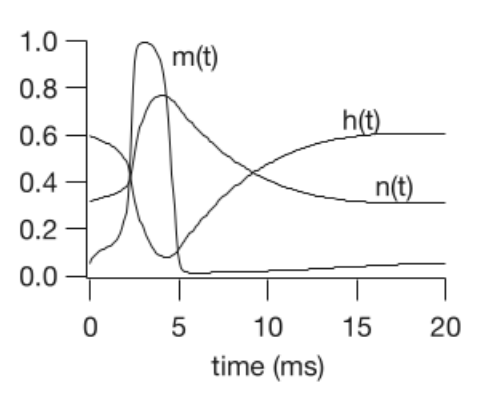
\includegraphics[height=5cm]{keener1.png}
	\caption{Gate Variables}
\end{subfigure}%
\begin{subfigure}{.5\textwidth}
	\centering
	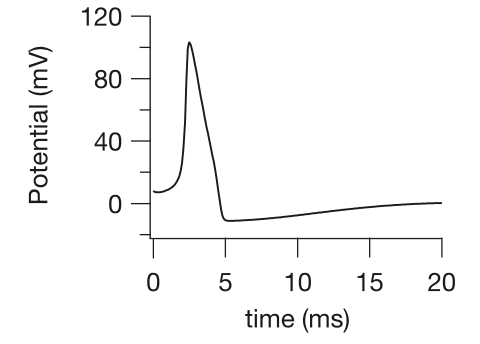
\includegraphics[height=5cm]{keener2.png}
	\caption{Action Potential}
\end{subfigure}
	\caption{Dynamics of H-H model Without Approximation on Shared Time-Scale (ms)}
	\label{fig:keen}
\end{figure}


Firstly, from Equation \ref{eq:time}, it's clear that the time constants, $\tau_i$ vary widely between these equations. For example, for a 20 mV potential, the values are $\tau_m \approx 0.4 ms$, $\tau_h \approx 8 ms$, and $\tau_n \approx 5 ms$. In general, it is true that $\tau_m$ is much smaller than the other time constants. Recall that $\tau_m$ is a measure of the speed with which $m$ converges to its steady state value $m_\infty$. Therefore, it may be a reasonable assumption to assume that $\tau_m$ is so fast compared to the other parameters that $m = m_\infty$. Then, we can either take $n$ or $h$ to be constant which would then give us a two-dimensional nonlinear system. Since $h$ fluctuates over the largest time-scale, we'll take it to be some constant $\bar{h}$. As a result, we have 

\begin{align*}
        C\frac{dV}{dt} &= I_{ext} -\bar{G}_{Na}m_\infty^3\bar{h}(V-E_{Na}) -\bar{G}_{K}n^4(V-E_{K})  -\bar{G}_{L}(V-E_{L}) \\
    \frac{dn}{dt} &= \frac{n_{\infty}-n}{\tau_n} 
\end{align*}

The assumption of taking $h$ to be constant can be judged visually in Figure \ref{fig:keen}, borrowed from Keener and Sneyd, which shows values of the unapproximated model\cite{keener}.

\begin{figure}
\centering
\begin{subfigure}{\textwidth}
	\centering
	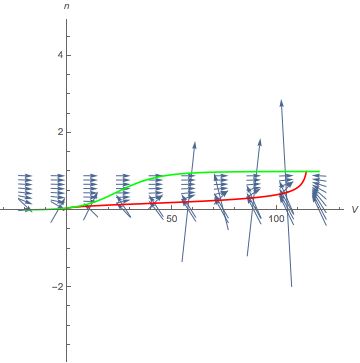
\includegraphics[width=10cm]{fastFast_nullc.png}
	\caption{$I_{ext}=0$ nullclines}
\end{subfigure}
\begin{subfigure}{\textwidth}
	\centering
	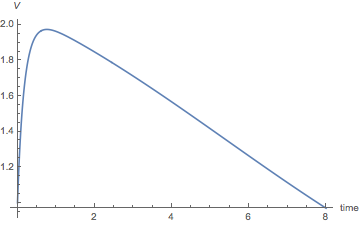
\includegraphics[width=10cm]{fastFast.png}
	\caption{$I_{ext}=0$ action potential}
\end{subfigure}
	\caption{V-nullcline (Red) and n-nullcline (Green) for $I_{ext}$ on and off of simple constant $h$ model, with associated action potentials}
	\label{fig:first}
\end{figure}

In Figure \ref{fig:first}, we see the result of our approximation. We can see that there are three potential intersections of the nullclines (two are present in the bottom left but difficult to visualize due to their close proximity), implying that there are excited and relaxed fixed points. If one looks closely at the vector field, the excited equilibrium (upper-right) appears to be attracting, and in the lower-left one equilibrium seems to be attracting while the other is a saddle. We'll call the one that is attracting in the lower-left the rest equilibrium, since it should correspond to the action potential going to rest. We also see that the action potential looks qualitatively different than it does in the unsimplified H-H model. The model seems less than ideal, but is a good initial step. 

We could treat $n$ and $h$ as bifurcation parameters. For example, we can use our physical intuition to consider the effects of increasing $n$ and decreasing $h$. Evidently, increasing $n$ corresponds to activation of K$^+$ conductance and deactivation of Na$^+$ conductance. As a result, we could predict the disappearance of the fixed point that corresponds to an excited state. Indeed, one can show that there is a saddle node bifurcation in this scenario resulting in the disappearance of the saddle and excited fixed points.\cite{keener} Instead of showing this, we'll seek a model that can provide genuine insight in the next section.

% Find fixed points (there are three)
% Find Jacobian and evaluate at these (should have 1 each of stable, unstable, saddle)

% Show that as I_ext increases we have (1) subcritical hopf bifurcation, then as it increases more (2) supercritical hopf bifurcation

% What this means is that initially the rest state is the most stable (so after an action potential, the nerve returns to rest). However, if we add some constant, external current, we can make a state of sustained action potentials stable. 

\section{Improving our Model}

\subsection{Derivation}

In our previous simplification, taking $m$ to converge infinitely fast to $m_\infty$ lent itself as a natural assumption due to its magnitude in speed relative to the other convergence speeds. However, taking $h$ to be constant seemed to be a shakier assumption, which was evaluated using Figure \ref{fig:keen}. However, one may have also observed, from the same figure, that there was some parity over $\approx 0.5$ that could be used. In other words, one could take the improved assumption that $n + h = 1$ which would imply that we could substitute $1 - n$ for $h$ rather than assuming that it is constant.

Evidently, this would give us

\begin{align*}
        C\frac{dV}{dt} &= I_{ext}-\bar{G}_{Na}m_\infty^3(1-n)(V-E_{Na}) -\bar{G}_{K}n^4(V-E_{K})  -\bar{G}_{L}(V-E_{L}) \\
    \frac{dn}{dt} &= \frac{n_{\infty}-n}{\tau_n} 
\end{align*}

\subsection{Phase Plane Analysis}

We can then begin our analysis the usual way, finding the nullclines to then find the fixed points. Hence, $\frac{dn}{dt}=0$ when $n_{\infty}=n$ and $\frac{dV}{dt}=0$ is satisfied when

\begin{align*}
        V &= \frac{\bar{G}_{Na}m_\infty^3(1-n)E_{Na}+\bar{G}_Kn^4E_K + G_LE_L + I_{ext}}{G_L + \bar{G}_{Na}m_\infty^3(1-n)+ \bar{G}_Kn^4}
\end{align*}

\begin{figure}
\centering
\begin{subfigure}{\textwidth}
	\centering
	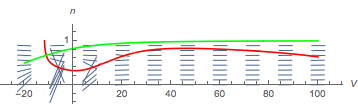
\includegraphics[width=10cm]{fast_slow_nullclines.png}
	\caption{$I_{ext}=0$ nullclines}
\end{subfigure}
\begin{subfigure}{\textwidth}
	\centering
	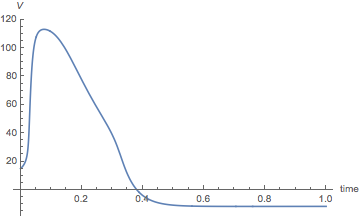
\includegraphics[width=8cm]{zero_ext_actionpotential.png}
	\caption{$I_{ext}=0$ action potential}
\end{subfigure}
\begin{subfigure}{\textwidth}
	\centering
	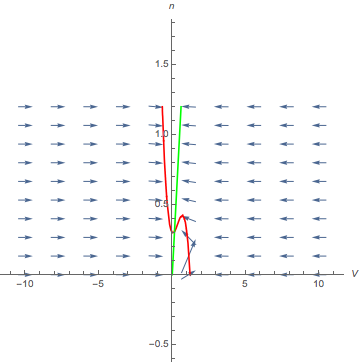
\includegraphics[width=5cm]{fast_slow_nullc_imp}
	\caption{$I_{ext}=50$ nullclines}
\end{subfigure}
\begin{subfigure}{\textwidth}
	\centering
	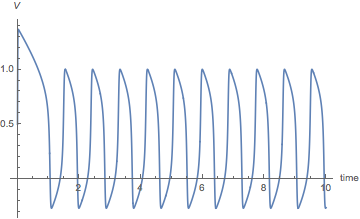
\includegraphics[width=8cm]{sustained_simple.png}
	\caption{$I_{ext}=50$ action potential}
\end{subfigure}
	\caption{V-nullcline (Red) and n-nullcline (Green) for $I_{ext}$ on and off of the $h=(1-n)$ model, with associated action potentials}
	\label{fig:nullc}
\end{figure}

Note that there is a divergence in kinetics observed by the variables in the system. In other words, because the Na$^+$ channel activates very quickly, $m$ and $V$ are fast variables. On the other hand, $n$ is slow because K$^+$ channels are activated slowly.\cite{keener} We observe this directly in the vector field shown in Figure \ref{fig:nullc} because the arrows specifying the trajectories in the phase plane are all nearly horizontal, except in the neighborhood of the $V$-nullcline. Note, then, that the implication is that solutions starting away from the $V$-nullcline will quickly move in a horizontal direction and therefore only observe the effect of $\frac{dn}{dt}$ when the solution is within a small neighborhood of the $V$-nullcline. 

Most interestingly, we observe that $I_{ext}$ shifts up the $V$-nullcline and produces sustained action potentials in response in Figure \ref{fig:nullc}.

Indeed, such behavior can be readily explained by this simplified model. It's at least clear that there is some sort of bifurcation being produced when $I_{ext}$ is in some critical range. When it is in this range, there must be an limit cycle oscillation (LCO) that becomes an attractor and therefore creates these sustained oscillations. 

First, note that the $V$-nullcline has a cubic shape, creating 3 branches (left, middle, right by increasing $V$). The branches are separated by the "elbows" or turning points in our cubic. Hence, because there are two elbows we have three regions. From the sign of $\frac{dV}{dt}$, it's clear that the middle branch is unstable and trajectories move toward the left and right branches.

Evidently, the interesting feature that explains the observed effect of $I_{ext}$ is hysteresis. Hence, consider the trajectory of the initial value which is perturbed enough to cross the middle branch, moving to the right branch of our V-nullcline and therefore governed by $dn/dt$ which is positive here. Hence, the solution will move up (the y-axis is $n$ so we should see movement up the y direction) the $V$-nullcline until it has a turning point. At this turning point, the solution will "jump across" to the left branch and the right branch will cease to exist. Then, on the left branch $dn/dt<0$ so the solution will begin to move down the $V$-nullcline (negative y-axis direction). Then, it will come across the equilibrium point (intersection with $n$-nullcline) and relax (completing the action potential). Of course, if it wasn't perturbed enough to cross the middle branch, then it would've just returned back to the stable point (and hence no action potential).

Impressively, this is the qualitative behavior we observe in action potentials with no external current, which is plotted in Figure \ref{fig:nullc}.

Now, it's clear why sustained potentials are realized when $I_{ext}$ is applied and in some proper range: The fixed point moves to the middle branch. Hence, consider our same example. The point begins on the right branch and travels with increasing $n$ until it reaches the turning point. Once it reaches the turning point, it jumps to the left branch and the right branch ceases to exist. However, the derivative ($dn/dt$) now flips signs and the solution begins to travel with decreasing $n$ until it reaches the turning point. Once it reaches this turning point, it jumps across to the right branch again, skipping over the fixed point entirely and continuing this process indefinitely!

\section{H-H and Relaxation Oscillations}

\subsection{Derivation}

We've shown that we can reduce the H-H model to a two-variable system that contains one slow and one fast variable and still capture important qualitative behavior. However, it seems that the important qualitative behavior that the model captured was mainly due to the cubic nullcline, which introduced hysteresis, and our consideration of the implications of having one fast and one slow variable. FitzHugh and Nagumo were similarly motivated by this reasoning after deriving a model similar to our previous one\cite{keener}. Hence, one can construct a system that retains the following essential properties:

\begin{enumerate}
    \item Two variables, one fast ($V$) and one slow ($n$)
    \item $V$ has a cubic nullcline and $n$ has a monotonically increasing nullcline
    \item nullclines have a single intersection point
\end{enumerate}

Hence, we can use the traditional FitzHugh-Nagumo system

\begin{align*}
    \epsilon {\dot  {V} }&= V(1-V)(V-\alpha) -n+I_{{{\rm {ext}}}} \\
     {\dot  {n}}&=V-\gamma n
\end{align*}

with $0<\alpha<1$ and $\epsilon << 1$. We'll take $\alpha = 0.1$, $\gamma = 0.5$, and $\epsilon = 0.01$ which gives us

\begin{align*}
    0.01 {\dot  {V} }&= V(1-V)(V-0.1) -n+I_{{{\rm {ext}}}} \\
     {\dot  {n}}&=V-0.5 n
\end{align*}

Notice that we chose $\epsilon$ to be small to ensure that $V$ is a fast variable and $n$ is a slow one. 

\subsection{Qualitative Discussion}

We can draw general conclusions before doing a rigorous analysis of this system. First, note that because $V$ is cubic we should have 3 branches of potential fixed points on our $V$-nullcline (which will not necessarily exist for all $n$). We'll say that these ranges are given by 

\begin{align*}
    V_l(n) \leq V_m(n) \leq V_r(n)
\end{align*}

It's clear too that our focus should be on these functions because our vector field is essentially horizontal everywhere (see Figure \ref{fig:nullc_nag}) that isn't in the neighborhood of the $V$-nullcline because we again made $V$ the fast variable and $n$ the slow one. 

We are under the assumption that our nullclines intersect at exactly one point. Hence, it must be true that our $n$-nullcline intersects with precisely one of these three branches. As we've seen before, the cubic has two elbows (turning points) at $V_l(n)=V_m(n)$ and at $V_r(n)=V_m(n)$ which results in the hysteresis we are now familiar with. So, we can observe that, if we've captured the characteristics we're interested in from our previous model properly and $\frac{dn}{dt}$ has the appropriate sign on $V_r(n)$ or $V_l(n)$, a fixed point on $V_r(n)$ or $V_l(n)$ should be stable and not so for $V_m(n)$. We can observe from Figure \ref{fig:nullc_nag} that this is indeed the case for at least one left-branch intersection (on $V_l(n)$). We'll prove this for the general case in our analytical discussion. 

Furthermore, we can see how hysteresis could occur from Figure \ref{fig:nullc_nag} as well. Indeed, if the fixed point lies on the middle branch we should see "relaxation oscillations" \cite{strog}. In other words, initial values will jump from the right to left branch and vis-versa for the same reasons discussed in the previous section, never reaching the fixed point and oscillating continuously. 

\begin{figure}
\centering
\begin{subfigure}{.5\textwidth}
	\centering
	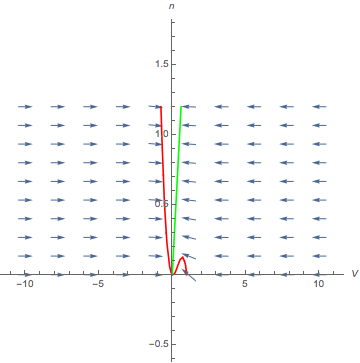
\includegraphics[width=5cm]{nullc_naguro.png}
	\caption{$I_{ext}=0$ nullclines}
\end{subfigure}%
\begin{subfigure}{.5\textwidth}
	\centering
	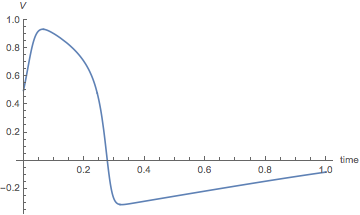
\includegraphics[width=5cm]{nagumo_ap.png}
	\caption{$I_{ext}=0$ action potential}
\end{subfigure}
\begin{subfigure}{.5\textwidth}
	\centering
	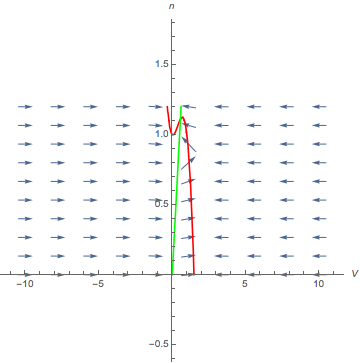
\includegraphics[width=5cm]{sustained_nagumo_nullc.png}
	\caption{$I_{ext}=0.1$ nullclines}
\end{subfigure}%
\begin{subfigure}{.5\textwidth}
	\centering
	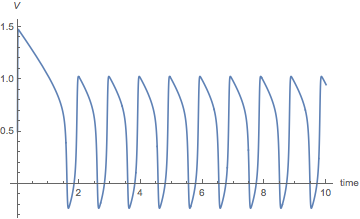
\includegraphics[width=5cm]{sustained_nagumo.png}
	\caption{$I_{ext}=0.1$ action potential}
\end{subfigure}
	\caption{V-nullcline (Red) and n-nullcline (Green) for $I_{ext}$ on and off of simple cubic model, with associated action potentials}
	\label{fig:nullc_nag}
\end{figure}

\subsection{Analytical and Numerical Discussion}

The Jacobian of the system with initial condition as above, $\alpha = 0.1$, $\gamma = 0.5$, and $\epsilon = 0.01$, is as follows.

\begin{align*}
J(V,n) &= \begin{bmatrix}
    -10(30v^2-22v+1)     & -100 \\
    1      & 0.5 \\
\end{bmatrix}
\end{align*}

Hence, the determinant, D, and trace, T are given by

\begin{align*}
D &= -5(30v^2-22v+1)+100 \\
T &= -\frac{1+20(30v^2-22v+1)}{2}
\end{align*}

Evidently, when $I_{ext}=0$ there is a fixed point at the origin which would then have

\begin{align*}
D &= 105 \\
T &= -\frac{1}{2}
\end{align*}

Evidently, this corresponds to a spiral sink. This is what our qualitative analysis would predict, as this relates to the fixed point lying on the left branch of the cubic nullcline, thus avoiding hysteresis and allowing the action potential to return to rest.

However, as $I_{ext}$ is introduced we'll see a shift in the location of our fixed point to the middle branch, where we'll find the same qualitative hysteresis behavior which is analytically an attracting limit cycle. Hence, we should be able to show the existence of a Hopf bifurcation. The general fixed point $(V_*, n_*)$ is given by the solution to 

\begin{align*}
0 &= 100[V_*(1-V_*)(V_*-0.1)-n_* + I_{ext}]\\
0 &= V-0.5n_*
\end{align*}

\begin{figure}
\centering
\begin{subfigure}{\textwidth}
	\centering
	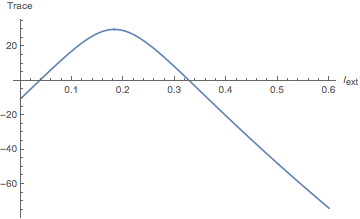
\includegraphics[width=10cm]{tr_ext.png}
	\caption{Trace of Jacobian in neighborhood of fixed point}
\end{subfigure}
\begin{subfigure}{\textwidth}
	\centering
	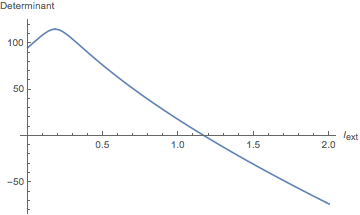
\includegraphics[width=10cm]{det_ext.png}
	\caption{Determinant of Jacobian in neighborhood of fixed point}
\end{subfigure}
	\caption{Linearization Analysis using Jacobian Matrix to Locate Hopf Bifurcations}
	\label{fig:det_tr}
\end{figure}

Hence, we can numerically compute this solution and plug it in directly to our trace and determinant equations derived above. The results are plotted in Figure \ref{fig:det_tr}. Evidently, we see that the trace flips sign twice in the range of $[0 mV,0.35 mV]$ of applied current, where the determinant is positive throughout this range so we can rule out a saddle point. This is expected because the trace first goes positive, indicating that the single fixed point, which was initially a spiral sink at the origin, loses stability which corresponds to the Hopf bifurcation where solutions tend toward a limit cycle oscillation as opposed to the fixed point. Later, when enough current is applied the fixed point gains stability again which corresponds to the fixed point moving to the right branch and the excited state becoming stable.

So, our bifurcation schematic would contain three regions

\begin{align*}
    \begin{cases}
    I_{ext} \in [\infty, 0.02] & \text{stable fixed point, left branch (rest)} \\
    I_{ext} \in [0.02, 0.33] &  \text{stable limit cycle, fixed point loses stability, middle branch} \\
    I_{ext} \in [0.33, \infty] & \text{stable fixed point, limit cycle loses stability, right branch (excited)}
    \end{cases}
\end{align*}

in agreement with our previous analyses. Note that 0.02 and 0.33 are our visual approximations and specific to this model (so the voltages don't match up necessarily with our other models). 

\subsection{Comparison with the True H-H Model}

\begin{figure}
\centering
	\centering
	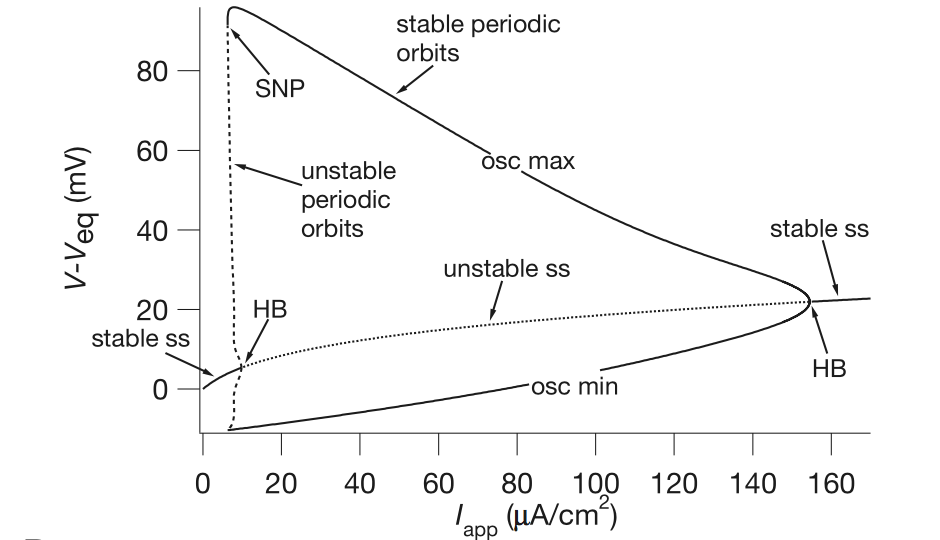
\includegraphics[width=10cm]{true.png}
	\caption{Bifurcation Diagram of Full H-H\cite{keener}}
	\label{fig:big_keen}
\end{figure}

Our analysis here, indicated the presence of two Hopf bifurcations. Now, we compare to a bifurcation diagram, taken from Keener and Sneyd, which shows the bifurcation properties of the H-H model across $I_{ext}$ shown in Figure \ref{fig:big_keen}. Evidently, the Hopf bifurcations are a true property of the system and limit cycle oscillations are present in a specific range of applied current. 

\section{Conclusion}

In summary, we derived the 4-dimensional H-H model in the same way that Hodgkin and Huxley did in their groundbreaking paper. We then looked to reduce the system to two dimensions. We initially tested an assumption that involved setting two gating variables constant. This allowed for us to observe equilibria that corresponded to rest and excited action potential state and predict a saddle-node bifurcation under applied current.

 We then, looked for a model that captured important qualitative behavior of the H-H model; namely, it's ability to Hopf bifurcate with applied current being the bifurcation parameter. This Hopf bifurcation was explained in terms of the hysteresis inherent to our cubic nullcline. Hence, when the single fixed point shifted to the middle branch it could never be reached by our perturbed system which would continue to oscillate with an attracting limit cycle. A second Hopf bifurcation occurred if enough current was applied, which implied the excited state becoming stable and reachable when the fixed point moved to the right branch of our cubic. 
 
 Finally, we turned to a less qualitative discussion by observing which aspects of our second model actually produced the behaviors we were interested in. Hence, we reduced our system to something reminiscent of a van der Pol oscillator and showed the same qualitative behaviors we found previously and then found the Hopf bifurcations analytically.
 
 Thankfully, the brave researchers who used numerical analysis to explicitly test our findings without approximation allows us to confirm the more qualitative results we found here in the sense that these Hopf bifurcations and action potentials are true phenomena observed in mathematics and in nature.\cite{monster}

\bibliography{nonlinear}
\bibliographystyle{plain}
\nocite{*}

\end{document}
